% Created by tikzDevice version 0.12.6 on 2026-07-04 06:01:28
% !TEX encoding = UTF-8 Unicode
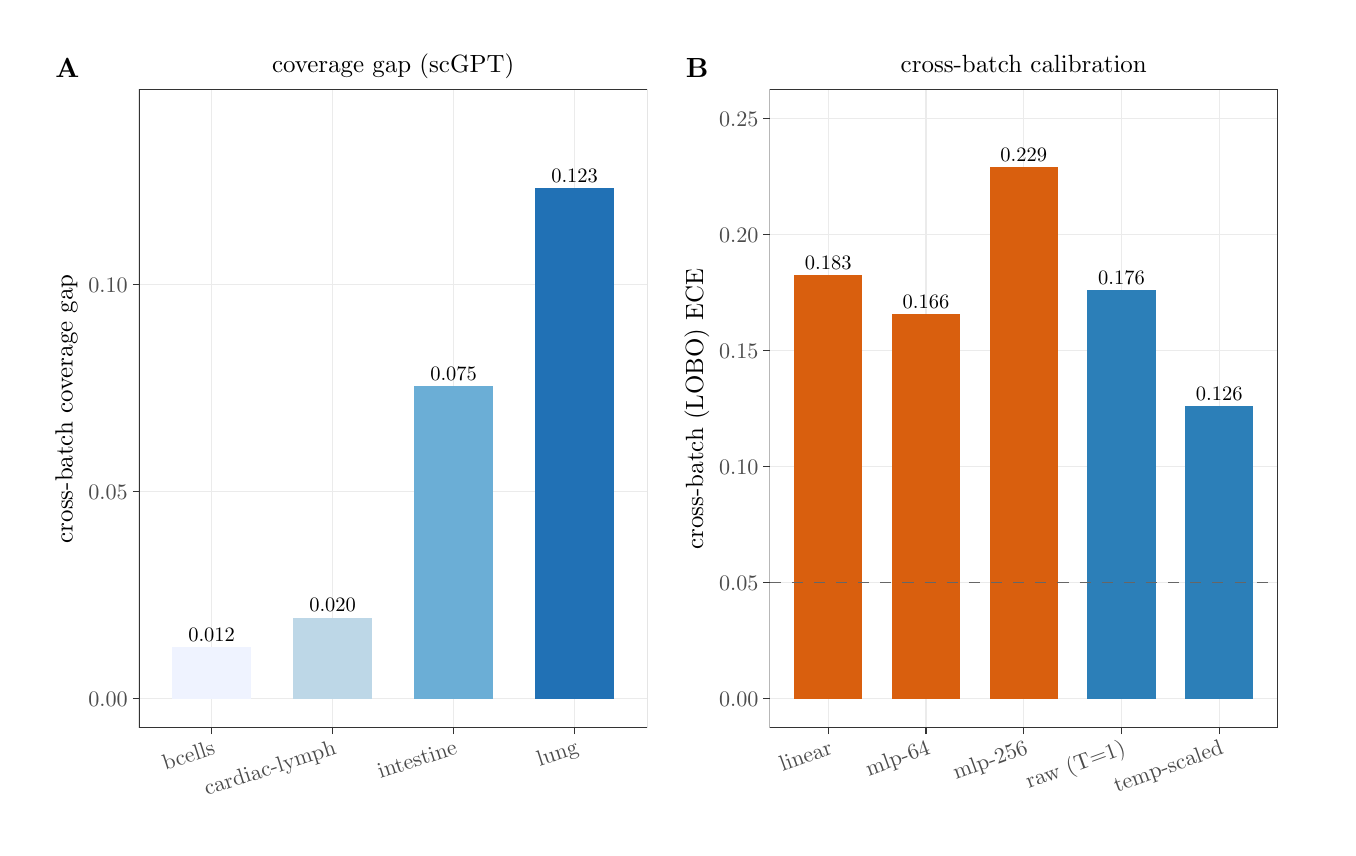
\begin{tikzpicture}[x=1pt,y=1pt]
\definecolor{fillColor}{RGB}{255,255,255}
\path[use as bounding box,fill=fillColor,fill opacity=0.00] (0,0) rectangle (469.75,289.08);
\begin{scope}
\path[clip] (  0.00,  0.00) rectangle (469.75,289.08);
\definecolor{drawColor}{RGB}{255,255,255}
\definecolor{fillColor}{RGB}{255,255,255}

\path[draw=drawColor,line width= 0.5pt,line join=round,line cap=round,fill=fillColor] (  0.00, -0.00) rectangle (469.75,289.08);
\end{scope}
\begin{scope}
\path[clip] (  5.00,  5.00) rectangle (232.88,284.08);
\definecolor{drawColor}{RGB}{255,255,255}
\definecolor{fillColor}{RGB}{255,255,255}

\path[draw=drawColor,line width= 0.5pt,line join=round,line cap=round,fill=fillColor] (  5.00,  5.00) rectangle (232.88,284.08);
\end{scope}
\begin{scope}
\path[clip] (232.88,  5.00) rectangle (460.75,284.08);
\definecolor{drawColor}{RGB}{255,255,255}
\definecolor{fillColor}{RGB}{255,255,255}

\path[draw=drawColor,line width= 0.5pt,line join=round,line cap=round,fill=fillColor] (232.88,  5.00) rectangle (460.76,284.08);
\end{scope}
\begin{scope}
\path[clip] ( 40.22, 36.09) rectangle (223.88,266.63);
\definecolor{fillColor}{RGB}{255,255,255}

\path[fill=fillColor] ( 40.22, 36.09) rectangle (223.88,266.63);
\definecolor{drawColor}{gray}{0.92}

\path[draw=drawColor,line width= 0.5pt,line join=round] ( 40.22, 46.57) --
	(223.88, 46.57);

\path[draw=drawColor,line width= 0.5pt,line join=round] ( 40.22,121.42) --
	(223.88,121.42);

\path[draw=drawColor,line width= 0.5pt,line join=round] ( 40.22,196.27) --
	(223.88,196.27);

\path[draw=drawColor,line width= 0.5pt,line join=round] ( 66.46, 36.09) --
	( 66.46,266.63);

\path[draw=drawColor,line width= 0.5pt,line join=round] (110.19, 36.09) --
	(110.19,266.63);

\path[draw=drawColor,line width= 0.5pt,line join=round] (153.91, 36.09) --
	(153.91,266.63);

\path[draw=drawColor,line width= 0.5pt,line join=round] (197.64, 36.09) --
	(197.64,266.63);
\definecolor{fillColor}{RGB}{33,113,181}

\path[fill=fillColor] (183.43, 46.57) rectangle (211.85,231.15);
\definecolor{fillColor}{RGB}{239,243,255}

\path[fill=fillColor] ( 52.25, 46.57) rectangle ( 80.67, 65.13);
\definecolor{fillColor}{RGB}{189,215,231}

\path[fill=fillColor] ( 95.97, 46.57) rectangle (124.40, 75.91);
\definecolor{fillColor}{RGB}{107,174,214}

\path[fill=fillColor] (139.70, 46.57) rectangle (168.12,159.59);
\definecolor{drawColor}{RGB}{0,0,0}

\node[text=drawColor,anchor=base,inner sep=0pt, outer sep=0pt, scale=  0.74] at (197.64,233.19) {0.123};

\node[text=drawColor,anchor=base,inner sep=0pt, outer sep=0pt, scale=  0.74] at ( 66.46, 67.17) {0.012};

\node[text=drawColor,anchor=base,inner sep=0pt, outer sep=0pt, scale=  0.74] at (110.19, 77.95) {0.020};

\node[text=drawColor,anchor=base,inner sep=0pt, outer sep=0pt, scale=  0.74] at (153.91,161.63) {0.075};
\definecolor{drawColor}{gray}{0.20}

\path[draw=drawColor,line width= 0.5pt,line join=round,line cap=round] ( 40.22, 36.09) rectangle (223.88,266.63);
\end{scope}
\begin{scope}
\path[clip] (  0.00,  0.00) rectangle (469.75,289.08);
\definecolor{drawColor}{gray}{0.30}

\node[text=drawColor,anchor=base east,inner sep=0pt, outer sep=0pt, scale=  0.80] at ( 36.17, 43.81) {0.00};

\node[text=drawColor,anchor=base east,inner sep=0pt, outer sep=0pt, scale=  0.80] at ( 36.17,118.66) {0.05};

\node[text=drawColor,anchor=base east,inner sep=0pt, outer sep=0pt, scale=  0.80] at ( 36.17,193.52) {0.10};
\end{scope}
\begin{scope}
\path[clip] (  0.00,  0.00) rectangle (469.75,289.08);
\definecolor{drawColor}{gray}{0.20}

\path[draw=drawColor,line width= 0.5pt,line join=round] ( 37.97, 46.57) --
	( 40.22, 46.57);

\path[draw=drawColor,line width= 0.5pt,line join=round] ( 37.97,121.42) --
	( 40.22,121.42);

\path[draw=drawColor,line width= 0.5pt,line join=round] ( 37.97,196.27) --
	( 40.22,196.27);
\end{scope}
\begin{scope}
\path[clip] (  0.00,  0.00) rectangle (469.75,289.08);
\definecolor{drawColor}{gray}{0.20}

\path[draw=drawColor,line width= 0.5pt,line join=round] ( 66.46, 33.84) --
	( 66.46, 36.09);

\path[draw=drawColor,line width= 0.5pt,line join=round] (110.19, 33.84) --
	(110.19, 36.09);

\path[draw=drawColor,line width= 0.5pt,line join=round] (153.91, 33.84) --
	(153.91, 36.09);

\path[draw=drawColor,line width= 0.5pt,line join=round] (197.64, 33.84) --
	(197.64, 36.09);
\end{scope}
\begin{scope}
\path[clip] (  0.00,  0.00) rectangle (469.75,289.08);
\definecolor{drawColor}{gray}{0.30}

\node[text=drawColor,rotate= 18.00,anchor=base east,inner sep=0pt, outer sep=0pt, scale=  0.80] at ( 68.16, 26.80) {bcells};

\node[text=drawColor,rotate= 18.00,anchor=base east,inner sep=0pt, outer sep=0pt, scale=  0.80] at (111.89, 26.80) {cardiac-lymph};

\node[text=drawColor,rotate= 18.00,anchor=base east,inner sep=0pt, outer sep=0pt, scale=  0.80] at (155.62, 26.80) {intestine};

\node[text=drawColor,rotate= 18.00,anchor=base east,inner sep=0pt, outer sep=0pt, scale=  0.80] at (199.34, 26.80) {lung};
\end{scope}
\begin{scope}
\path[clip] (  0.00,  0.00) rectangle (469.75,289.08);
\definecolor{drawColor}{RGB}{0,0,0}

\node[text=drawColor,rotate= 90.00,anchor=base,inner sep=0pt, outer sep=0pt, scale=  0.90] at ( 16.20,151.36) {cross-batch coverage gap};
\end{scope}
\begin{scope}
\path[clip] (  0.00,  0.00) rectangle (469.75,289.08);
\definecolor{drawColor}{RGB}{0,0,0}

\node[text=drawColor,anchor=base,inner sep=0pt, outer sep=0pt, scale=  0.90] at (132.05,272.88) {coverage gap (scGPT)};
\end{scope}
\begin{scope}
\path[clip] (  0.00,  0.00) rectangle (469.75,289.08);
\definecolor{drawColor}{RGB}{0,0,0}

\node[text=drawColor,anchor=base,inner sep=0pt, outer sep=0pt, scale=  1.00] at ( 14.35,271.12) {\bfseries A};
\end{scope}
\begin{scope}
\path[clip] (268.10, 36.09) rectangle (451.75,266.63);
\definecolor{fillColor}{RGB}{255,255,255}

\path[fill=fillColor] (268.10, 36.09) rectangle (451.75,266.63);
\definecolor{drawColor}{gray}{0.92}

\path[draw=drawColor,line width= 0.5pt,line join=round] (268.10, 46.57) --
	(451.75, 46.57);

\path[draw=drawColor,line width= 0.5pt,line join=round] (268.10, 88.49) --
	(451.75, 88.49);

\path[draw=drawColor,line width= 0.5pt,line join=round] (268.10,130.40) --
	(451.75,130.40);

\path[draw=drawColor,line width= 0.5pt,line join=round] (268.10,172.32) --
	(451.75,172.32);

\path[draw=drawColor,line width= 0.5pt,line join=round] (268.10,214.23) --
	(451.75,214.23);

\path[draw=drawColor,line width= 0.5pt,line join=round] (268.10,256.15) --
	(451.75,256.15);

\path[draw=drawColor,line width= 0.5pt,line join=round] (289.29, 36.09) --
	(289.29,266.63);

\path[draw=drawColor,line width= 0.5pt,line join=round] (324.61, 36.09) --
	(324.61,266.63);

\path[draw=drawColor,line width= 0.5pt,line join=round] (359.93, 36.09) --
	(359.93,266.63);

\path[draw=drawColor,line width= 0.5pt,line join=round] (395.25, 36.09) --
	(395.25,266.63);

\path[draw=drawColor,line width= 0.5pt,line join=round] (430.56, 36.09) --
	(430.56,266.63);
\definecolor{fillColor}{RGB}{217,95,14}

\path[fill=fillColor] (276.93, 46.57) rectangle (301.65,199.82);

\path[fill=fillColor] (312.25, 46.57) rectangle (336.97,185.56);

\path[fill=fillColor] (347.57, 46.57) rectangle (372.29,238.63);
\definecolor{fillColor}{RGB}{44,127,184}

\path[fill=fillColor] (382.88, 46.57) rectangle (407.61,194.28);

\path[fill=fillColor] (418.20, 46.57) rectangle (442.93,152.37);
\definecolor{drawColor}{RGB}{0,0,0}

\node[text=drawColor,anchor=base,inner sep=0pt, outer sep=0pt, scale=  0.74] at (289.29,201.85) {0.183};

\node[text=drawColor,anchor=base,inner sep=0pt, outer sep=0pt, scale=  0.74] at (324.61,187.60) {0.166};

\node[text=drawColor,anchor=base,inner sep=0pt, outer sep=0pt, scale=  0.74] at (359.93,240.67) {0.229};

\node[text=drawColor,anchor=base,inner sep=0pt, outer sep=0pt, scale=  0.74] at (395.25,196.32) {0.176};

\node[text=drawColor,anchor=base,inner sep=0pt, outer sep=0pt, scale=  0.74] at (430.56,154.41) {0.126};
\definecolor{drawColor}{gray}{0.40}

\path[draw=drawColor,line width= 0.5pt,dash pattern=on 4pt off 4pt ,line join=round] (268.10, 88.49) -- (451.75, 88.49);
\definecolor{drawColor}{gray}{0.20}

\path[draw=drawColor,line width= 0.5pt,line join=round,line cap=round] (268.10, 36.09) rectangle (451.75,266.63);
\end{scope}
\begin{scope}
\path[clip] (  0.00,  0.00) rectangle (469.75,289.08);
\definecolor{drawColor}{gray}{0.30}

\node[text=drawColor,anchor=base east,inner sep=0pt, outer sep=0pt, scale=  0.80] at (264.05, 43.81) {0.00};

\node[text=drawColor,anchor=base east,inner sep=0pt, outer sep=0pt, scale=  0.80] at (264.05, 85.73) {0.05};

\node[text=drawColor,anchor=base east,inner sep=0pt, outer sep=0pt, scale=  0.80] at (264.05,127.65) {0.10};

\node[text=drawColor,anchor=base east,inner sep=0pt, outer sep=0pt, scale=  0.80] at (264.05,169.56) {0.15};

\node[text=drawColor,anchor=base east,inner sep=0pt, outer sep=0pt, scale=  0.80] at (264.05,211.48) {0.20};

\node[text=drawColor,anchor=base east,inner sep=0pt, outer sep=0pt, scale=  0.80] at (264.05,253.40) {0.25};
\end{scope}
\begin{scope}
\path[clip] (  0.00,  0.00) rectangle (469.75,289.08);
\definecolor{drawColor}{gray}{0.20}

\path[draw=drawColor,line width= 0.5pt,line join=round] (265.85, 46.57) --
	(268.10, 46.57);

\path[draw=drawColor,line width= 0.5pt,line join=round] (265.85, 88.49) --
	(268.10, 88.49);

\path[draw=drawColor,line width= 0.5pt,line join=round] (265.85,130.40) --
	(268.10,130.40);

\path[draw=drawColor,line width= 0.5pt,line join=round] (265.85,172.32) --
	(268.10,172.32);

\path[draw=drawColor,line width= 0.5pt,line join=round] (265.85,214.23) --
	(268.10,214.23);

\path[draw=drawColor,line width= 0.5pt,line join=round] (265.85,256.15) --
	(268.10,256.15);
\end{scope}
\begin{scope}
\path[clip] (  0.00,  0.00) rectangle (469.75,289.08);
\definecolor{drawColor}{gray}{0.20}

\path[draw=drawColor,line width= 0.5pt,line join=round] (289.29, 33.84) --
	(289.29, 36.09);

\path[draw=drawColor,line width= 0.5pt,line join=round] (324.61, 33.84) --
	(324.61, 36.09);

\path[draw=drawColor,line width= 0.5pt,line join=round] (359.93, 33.84) --
	(359.93, 36.09);

\path[draw=drawColor,line width= 0.5pt,line join=round] (395.25, 33.84) --
	(395.25, 36.09);

\path[draw=drawColor,line width= 0.5pt,line join=round] (430.56, 33.84) --
	(430.56, 36.09);
\end{scope}
\begin{scope}
\path[clip] (  0.00,  0.00) rectangle (469.75,289.08);
\definecolor{drawColor}{gray}{0.30}

\node[text=drawColor,rotate= 20.00,anchor=base east,inner sep=0pt, outer sep=0pt, scale=  0.80] at (291.18, 26.86) {linear};

\node[text=drawColor,rotate= 20.00,anchor=base east,inner sep=0pt, outer sep=0pt, scale=  0.80] at (326.49, 26.86) {mlp-64};

\node[text=drawColor,rotate= 20.00,anchor=base east,inner sep=0pt, outer sep=0pt, scale=  0.80] at (361.81, 26.86) {mlp-256};

\node[text=drawColor,rotate= 20.00,anchor=base east,inner sep=0pt, outer sep=0pt, scale=  0.80] at (397.13, 26.86) {raw (T=1)};

\node[text=drawColor,rotate= 20.00,anchor=base east,inner sep=0pt, outer sep=0pt, scale=  0.80] at (432.45, 26.86) {temp-scaled};
\end{scope}
\begin{scope}
\path[clip] (  0.00,  0.00) rectangle (469.75,289.08);
\definecolor{drawColor}{RGB}{0,0,0}

\node[text=drawColor,rotate= 90.00,anchor=base,inner sep=0pt, outer sep=0pt, scale=  0.90] at (244.08,151.36) {cross-batch (LOBO) ECE};
\end{scope}
\begin{scope}
\path[clip] (  0.00,  0.00) rectangle (469.75,289.08);
\definecolor{drawColor}{RGB}{0,0,0}

\node[text=drawColor,anchor=base,inner sep=0pt, outer sep=0pt, scale=  0.90] at (359.93,272.88) {cross-batch calibration};
\end{scope}
\begin{scope}
\path[clip] (  0.00,  0.00) rectangle (469.75,289.08);
\definecolor{drawColor}{RGB}{0,0,0}

\node[text=drawColor,anchor=base,inner sep=0pt, outer sep=0pt, scale=  1.00] at (241.97,271.12) {\bfseries B};
\end{scope}
\end{tikzpicture}
